
\documentclass[]{beamer}
%\includeonlyframes{current} Does not work, though
\mode<presentation>{
\usefonttheme{professionalfonts}
\useinnertheme{rounded}
\useoutertheme[subsection=false,footline=authortitle]{miniframes}
%Inner Color Themes
\usecolortheme{dolphin}
%	\usecolortheme{seahorse}


%Outer Color Themes
\usecolortheme{rose}
%\usecolortheme{orchid}
}

%Typical documenttypes: article/book
%some examples:
%\documentclass[reqno,11pt]{book}   %%%for books
%\documentclass[]{minimal}			%%%for Minimal Working Example






%%%%%%%%%%%%%%%%%%%% setting for fast compiling

%\special{dvipdfmx:config z 0}		% no compression

\includeonly{chapters/chapter9}		% In practice, use an empty document called "chapter9"	% usually for printing books






%%%%%%%%%%%%%%%%%%%% here we include packages

%%%basic packages for math articles
\usepackage{amssymb}
\usepackage{amsthm}
\usepackage{amsmath}
\usepackage{amsfonts}
%\usepackage[shortlabels]{enumitem}	% It supersedes both enumerate and mdwlist. The package option shortlabels is included to configure the labels like in enumerate.

%%%packages for special symbols
\usepackage{pifont}					% Access to PostScript standard Symbol and Dingbats fonts
\usepackage{wasysym}				% additional characters
\usepackage{bm}						% bold fonts: \bm{...}
\usepackage{extarrows}				% may be replaced by tikz-cd
%\usepackage{unicode-math}			% unicode maths for math fonts, now I don't know how to include it

%%%basic packages for fancy electronic documents
%\usepackage[colorlinks]{hyperref}
%\usepackage[table,hyperref]{xcolor} 			% before tikz-cd. 
%\usepackage[table,hyperref,monochrome]{xcolor}	% disable colored output (black and white)

%%%packages for figures and tables (general setting)
\usepackage{float}				%Improved interface for floating objects
\usepackage{caption,subcaption}
\usepackage{adjustbox}			% for me it is usually used in tables 
\usepackage{stackengine}		%baseline changes

%%%packages for commutative diagrams
\usepackage{tikz-cd}
%\usepackage{quiver}			% see https://q.uiver.app/

%%%packages for pictures
\usepackage[width=0.5,tiewidth=0.7]{strands}
\usepackage{graphicx}			% Enhanced support for graphics

%%%packages for tables and general settings
\usepackage{array}
\usepackage{makecell}
\usepackage{multicol}
\usepackage{multirow}
\usepackage{diagbox}



%%%packages for temporary usage
\usepackage{mathtools}
\usepackage{tabularx}
\usepackage{etoolbox}



%https://tex.stackexchange.com/questions/58852/possible-incompatibility-with-enumitem










%%%%%%%%%%%%%%%%%%%% here we include theoremstyles

\numberwithin{equation}{section}

\theoremstyle{plain}
%\newtheorem{theorem}{Theorem}[section]

\newtheorem{setting}[theorem]{Setting}
%\newtheorem{definition}[theorem]{Definition}
%\newtheorem{lemma}[theorem]{Lemma}
\newtheorem{proposition}[theorem]{Proposition}
%\newtheorem{corollary}[theorem]{Corollary}
\newtheorem{conjecture}[theorem]{Conjecture}

\newtheorem{claim}[theorem]{Claim}
\newtheorem{eg}[theorem]{Example}
\newtheorem{ex}[theorem]{Exercise}
%\newtheorem{fact}[theorem]{Fact}
\newtheorem{ques}[theorem]{Question}
\newtheorem{warning}[theorem]{Warning}



\newtheorem*{bbox}{Black box}
\newtheorem*{notation}{Conventions and Notations}


\numberwithin{equation}{section}


\theoremstyle{remark}

\newtheorem{remark}[theorem]{Remark}
\newtheorem*{remarks}{Remarks}

%%% for important theorems
%\newtheoremstyle{theoremletter}{4mm}{1mm}{\itshape}{ }{\bfseries}{}{ }{}
%\theoremstyle{theoremletter}
%\newtheorem{theoremA}{Theorem}
%\renewcommand{\thetheoremA}{A}
%\newtheorem{theoremB}{Theorem}
%\renewcommand{\thetheoremB}{B}

\newtheorem{short}{ }





%%%%%%%%%%%%%%%%%%%% here we declare some symbols

%%%%%%%DeclareMathOperator
%see here for why newcommand is better for DeclareMathOperator: https://tex.stackexchange.com/questions/67506/newcommand-vs-declaremathoperator

%%%%%basic symbols. Keep them!

%%%symbols for sets and maps
\DeclareMathOperator{\pt}{\{\ast\}}	%points. Other possibilities are \{pt\}, \{*\}...
\DeclareMathOperator{\Id}{\operatorname{Id}}	%identity in groups.
\DeclareMathOperator{\Img}{\operatorname{Im}}

\DeclareMathOperator{\Ob}{\operatorname{Ob}}
\DeclareMathOperator{\Mor}{\operatorname{Mor}}	%difference of Mor and Hom: Hom is usually for abelian categories
\DeclareMathOperator{\Hom}{\operatorname{Hom}}	\DeclareMathOperator{\End}{\operatorname{End}}
\DeclareMathOperator{\Aut}{\operatorname{Aut}}

%%%symbols for linear algebras and 
%%linear algebras
\DeclareMathOperator{\tr}{\operatorname{tr}}
\DeclareMathOperator{\diag}{\operatorname{diag}}	%for diagonal matrices

%%abstract algebras
\DeclareMathOperator{\ord}{\operatorname{ord}}
\DeclareMathOperator{\gr}{\operatorname{gr}}
\DeclareMathOperator{\Frac}{\operatorname{Frac}}

%%%symbols for basic geometries
\DeclareMathOperator{\vol}{\operatorname{vol}}	%volume
\DeclareMathOperator{\dist}{\operatorname{dist}}
\DeclareMathOperator{\supp}{\operatorname{supp}}

%%%symbols for category
%%names of categories
\DeclareMathOperator{\Mod}{\operatorname{Mod}}
\DeclareMathOperator{\Vect}{\operatorname{Vect}}
\DeclareMathOperator{\rep}{\operatorname{rep}} %usually rep means the category of finite dimensional representations, while Rep means the category of representations.
\DeclareMathOperator{\Rep}{\operatorname{Rep}}


%%%symbols for homological algebras
\DeclareMathOperator{\Tor}{\operatorname{Tor}}
\DeclareMathOperator{\Ext}{\operatorname{Ext}}
\DeclareMathOperator{\gldim}{\operatorname{gl.dim}}
\DeclareMathOperator{\projdim}{\operatorname{proj.dim}}
\DeclareMathOperator{\injdim}{\operatorname{inj.dim}}
\DeclareMathOperator{\rad}{\operatorname{rad}}


%%%symbols for algebraic groups
\DeclareMathOperator{\GL}{\operatorname{GL}}
\DeclareMathOperator{\SL}{\operatorname{SL}}

%%%symbols for typical varieties
\DeclareMathOperator{\Gr}{\operatorname{Gr}}
\DeclareMathOperator{\Flag}{\operatorname{Flag}}

%%%symbols for basic algebraic geometry
\DeclareMathOperator{\Spec}{\operatorname{Spec}}
\DeclareMathOperator{\Coh}{\operatorname{Coh}}
\newcommand{\Dcoh}{\mathcal{D}_{\operatorname{Coh}}}%%%This one shows the difference between \DeclareMathOperator and \newcommand
\DeclareMathOperator{\Pic}{\operatorname{Pic}}
\DeclareMathOperator{\Jac}{\operatorname{Jac}}

%%%%%advanced symbols. Choose the part you need!

%%%symbols for algebraic representation theory
\DeclareMathOperator{\Irr}{\operatorname{Irr}}
\DeclareMathOperator{\ind}{\operatorname{ind}}	%\ind(Q) means the set of  equivalence classes of finite dimensional indecomposable representations
\DeclareMathOperator{\Res}{\operatorname{Res}}
\DeclareMathOperator{\Ind}{\operatorname{Ind}}
\DeclareMathOperator{\cInd}{\operatorname{c-Ind}}


%%%symbols for algebraic topology
\DeclareMathOperator{\EGG}{\operatorname{E}\!}
\DeclareMathOperator{\BGG}{\operatorname{B}\!}

\DeclareMathOperator{\chern}{\operatorname{ch}^{*}}
\DeclareMathOperator{\Td}{\operatorname{Td}}
\DeclareMathOperator{\AS}{\operatorname{AS}}	%Atiyah--Segal completion theorem 

%%%symbols for Auslander--Reiten theory 
\DeclareMathOperator{\Modup}{\overline{\operatorname{mod}}}
\DeclareMathOperator{\Moddown}{\underline{\operatorname{mod}}}
\DeclareMathOperator{\Homup}{\overline{\operatorname{Hom}}}
\DeclareMathOperator{\Homdown}{\underline{\operatorname{Hom}}}


%%%symbols for operad
\DeclareMathOperator{\Com}{\operatorname{\mathcal{C}om}}
\DeclareMathOperator{\Ass}{\operatorname{\mathcal{A}ss}}
\DeclareMathOperator{\Lie}{\operatorname{\mathcal{L}ie}}
\DeclareMathOperator{\calEnd}{\operatorname{\mathcal{E}nd}} %cal=\mathcal


%%%%%personal symbols. Use at your own risk!

%%%symbols only for master thesis
\DeclareMathOperator{\ptt}{\operatorname{par}}	%the partition map
\DeclareMathOperator{\str}{\operatorname{str}}	%strict case
\DeclareMathOperator{\RRep}{\widetilde{\operatorname{Rep}}}
\DeclareMathOperator{\Rpt}{\operatorname{R}}
\DeclareMathOperator{\Rptc}{\operatorname{\mathcal{R}}}
\DeclareMathOperator{\Spt}{\operatorname{S}}
\DeclareMathOperator{\Sptc}{\operatorname{\mathcal{S}}}
\DeclareMathOperator{\Kcurl}{\operatorname{\mathcal{K}}}
\DeclareMathOperator{\Hcurl}{\operatorname{\mathcal{H}}}
\DeclareMathOperator{\eu}{\operatorname{eu}}
\DeclareMathOperator{\Eu}{\operatorname{Eu}}
\DeclareMathOperator{\dimv}{\operatorname{\underline{\mathbf{dim}}}}
\DeclareMathOperator{\St}{\mathcal{Z}}

%%%%%symbols which haven't been classified. Add your own math operators here!


\DeclareMathOperator{\Modr}{\operatorname{-Mod}}
\DeclareMathOperator{\BM}{\operatorname{BM}}




%%%%%%%newcommand

%%%basic symbols
\newcommand{\norm}[1]{\Vert{#1}\Vert}

%%%symbols only for master thesis
\newcommand{\dimvec}[1]{\mathbf{#1}}
\newcommand{\abdimvec}[1]{|\dimvec{#1}|}
\newcommand{\ftdimvec}[1]{\underline{\dimvec{#1}}}

\newcommand{\absgp}[1]{\mathbb{#1}}
\newcommand{\WWd}{\absgp{W}_{\abdimvec{d}}}
\newcommand{\Wd}{W_{\dimvec{d}}}
\newcommand{\ww}{\varpi}
\newcommand{\MinWd}{\operatorname{Min}(\absgp{W}_{\abdimvec{d}},W_{\dimvec{d}})}
\newcommand{\Compd}{\operatorname{Comp}_{\dimvec{d}}}
\newcommand{\Shuffled}{\operatorname{Shuffle}_{\dimvec{d}}}


\newcommand{\Omcell}{\Omega}
\newcommand{\OOmcell}{\boldsymbol{\Omega}}
\newcommand{\Vcell}{\mathcal{V}}
\newcommand{\VVcell}{\boldsymbol{\mathcal{V}}}
\newcommand{\Ocell}{\mathcal{O}}
\newcommand{\OOcell}{\boldsymbol{\mathcal{O}}}
\newcommand{\preimage}[1]{\widetilde{#1}}
\newcommand{\orde}{\operatorname{ord}_e}
\newcommand{\fakestar}{*}

%as the subscription of Hom
\newcommand{\Alggp}{\text{-Alg gp}}


%%%%%symbols which haven't been determined. Add your own math operators here!
\newcommand{\Flagbra}[1]{\Flag_{(#1)}}



%%%%%%%%%%%%%%%%%%%% here we make some blocks for special features. 

%%%% todo notes %%%%
\usepackage[colorinlistoftodos,textsize=footnotesize]{todonotes}
\setlength{\marginparwidth}{2.5cm}
\newcommand{\leftnote}[1]{\reversemarginpar\marginnote{\footnotesize #1}}
\newcommand{\rightnote}[1]{\normalmarginpar\marginnote{\footnotesize #1}\reversemarginpar}


%%%% Show outline around overlayarea %%%%
%https://tex.stackexchange.com/questions/573822/show-outline-around-overlayarea
\makeatletter
\newif\ifbeamer@show@overlayarea
\pgfkeys{/beamer/overlayarea/.cd,show frame/.is if=beamer@show@overlayarea,
show frame/.default=true}
\beamer@show@overlayareafalse
\mode
<presentation>
{\renewenvironment{overlayarea}[3][]{%
  \pgfkeys{/beamer/overlayarea/.cd,#1}%
  \beamer@animht=#2\relax
  \beamer@animwd=#3\relax
  \setbox\beamer@areabox=\vbox to\beamer@animwd\bgroup
  \strut\begin{minipage}[t]{\beamer@animht}%
  % Make the minipage behave like the main part of the slide
  \normalfont
  \raggedright
  }
  {%
  \end{minipage}\endgraf\vfil
  \egroup
  \wd\beamer@areabox=\beamer@animht
  \ht\beamer@areabox=\beamer@animwd
  \dp\beamer@areabox=0pt %
  \ifbeamer@show@overlayarea
   \bgroup\fboxsep=0pt\relax
   \hspace*{-0.4pt}\vspace*{-0.4pt}%
   \fbox{\box\beamer@areabox}\hspace*{-0.4pt}\vspace*{-0.4pt}%
   \egroup
  \else
   \box\beamer@areabox
  \fi 
}}
\makeatother





%%%%%%%%%%%%%%%%%%%% here we make some global settings. Understand everything here before you make a document!

%\usepackage[a4paper,left=3cm,right=3cm,bottom=4cm]{geometry}
%\usepackage{indentfirst}	% Indent first paragraph after section header

\setcounter{tocdepth}{2}


%https://latexref.xyz/_005cparindent-_0026-_005cparskip.html
\setlength{\parindent}{15pt}	
\setlength{\parskip}{0pt plus1pt}
\patchcmd{\smallmatrix}{\thickspace}{\kern.2mm}{}{}
%\setlength\intextsep{0cm}
%\setlength\textfloatsep{0cm}
\def\arraystretch{1}
%\setcounter{secnumdepth}{3}

\allowdisplaybreaks
\newcommand\scalemath[2]{\scalebox{#1}{$\displaystyle #2$}}

%https://tex.stackexchange.com/questions/315996/how-to-use-includeonlyframes-with-textblock-all-pages-are-printed
%\makeatletter
%\patchcmd{\beamer@@@@frame}% <cmd>
%  {\setkeys{beamerframe}{#2}}% <search>
%  {\edef\theframe{\number\numexpr\value{framenumber}+1}%
%   \setkeys{beamerframe}{label=frame-\theframe,#2}}% <replace>
%  {}{}% <success><failure>
%\makeatother


% 设置图形文件的搜索路径


\graphicspath{{../figures/}}

\usepackage[T1]{fontenc}




\begin{document}
% The beginning depends on the documentclass. Rewrite this part if you use different documentclass!


\title{Affine pavings of partial flag varieties}
\author[Xiaoxiang Zhou]{Xiaoxiang Zhou\\[10mm]{\small Advisor: Prof. Dr. Catharina Stroppel \\ Second Advisor: Dr. Jens Niklas Eberhardt}}
\institute[Bonn uni]{Universität Bonn}
\date{\today}

\begin{frame}
\titlepage
\end{frame}
\begin{frame}{Process}
\tableofcontents[hideallsubsections]
\end{frame}
\section{Setting and Statement}
\begin{frame}{Process}
\tableofcontents[currentsection,hideallsubsections]
\end{frame}
\begin{frame}[fragile]{Affine paving}
\begin{setting}
$K= \mathbb{C}$, $X$: algebraic variety over $K$. 
\end{setting}
\begin{definition}
An \textbf{affine paving} of $X$ is a filtration
$$0= X_0 \subset X_1 \subset \cdots \subset X_d=X$$
with $X_i$ closed and $X_{i+1} \smallsetminus X_i \cong \mathbb{A}^k_{K}$.
\end{definition}
\begin{figure}[th]
\begin{minipage}[b]{.45\textwidth}
	\centering
	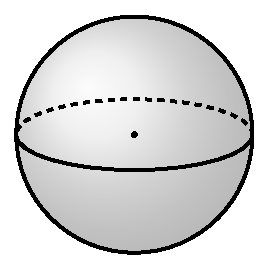
\includegraphics[width=.3\textwidth]{figures/sphere/Sphere1.pdf}
	$$\mathbb{P}^1= \{ \infty \} \sqcup \mathbb{A}^1$$
\end{minipage}
\begin{minipage}[b]{.45\textwidth}
\centering
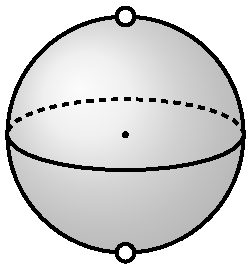
\includegraphics[width=.3\textwidth]{figures/sphere/Sphere3.pdf}
$$\mathbb{P}^1 \smallsetminus \{0,\infty \} \text{ has no affine paving}$$
\end{minipage}
\end{figure}

\end{frame}

\begin{frame}[fragile]{Quiver and quiver representation}

Quiver is a graph. It has some vertices $\&$ arrows.\\

In this talk, all the quivers are finite and connected.

\end{frame}

\begin{frame}[fragile]{Quiver and quiver representation}

We focus on the Dynkin quiver.\\

That means, the graph of the Dynkin diagrams in the ADE series.

\end{frame}

%https://tex.stackexchange.com/questions/436284/how-to-adjust-parenthesis-thickness-without-changing-the-font
%https://tex.stackexchange.com/questions/207056/wrong-too-much-vertical-space-above-vdots-in-small-matrix
\begin{frame}[fragile]{Partial flag variety}
\begin{definition}
Fix a quiver $Q$ and $M \in \rep(Q)$,
\begin{equation*}
\begin{aligned}
\Flag_{d}(M)\colon=\;& \left\{ F\colon 0 \subseteq N_1 \subseteq \cdots\subseteq N_d \subseteq M  \right\} \\ 
\Flag_{\ftdimvec{f}}(M)\colon=\;&\left\{ F\colon 0 \subseteq N_1 \subseteq \cdots\subseteq N_d \subseteq M \;\middle|\;\rule{0mm}{3.4mm} \dimv M_i =\ftdimvec{f}_i \right\}
\end{aligned}
\end{equation*}
\end{definition}
\begin{eg}
$Q= \bullet$, $M=\mathbb{C}^n$, $\ftdimvec{f}:=\scalemath{0.7}
{\left(
\begin{smallmatrix}
\scriptsize n \\ \vphantom{\int\limits^x}\smash{\vdots} \\ 1
\end{smallmatrix}
\right)}$
\begin{equation*}
\begin{aligned}
\Flag_{d}(\mathbb{C}^n)=\;& \left\{ F\colon 0 \subseteq N_1 \subseteq \cdots\subseteq N_d \subseteq \mathbb{C}^n  \right\}\hspace{-10mm}& \\ 
\Flag_{1}(\mathbb{C}^n)=\;& \left\{ F\colon 0 \subseteq N_1  \subseteq \mathbb{C}^n  \right\} &= \sqcup_{k=0}^{n} \Gr (n,k) \\
\Flag_{\ftdimvec{f}}(\mathbb{C}^n)=\;&\text{ complete flags of $\mathbb{C}^n$} & \\
\Flag_{(\!k\!)}\!(\mathbb{C}^n)=\;& \Gr (n,k) &\\
\end{aligned}
\end{equation*}
\end{eg}

\end{frame}


\begin{frame}[fragile]{Statement}
\begin{theorem}
For a Dynkin quiver $Q$ and $M \in \rep(Q)$, 
$$\Flag_{d}(M) \text{ has an affine paving.}$$
\end{theorem}

\end{frame}


%%%%%%%%%%%%%%%%%%%%%%%%%%%%%%%%%%%%
\section{Case study}
\begin{frame}{Process}
\tableofcontents[currentsection,hideallsubsections]
\end{frame}


\begin{frame}[fragile]{Task 1. $Q= \bullet$, $M=\mathbb{C}^n$}

In this case,
% https://q.uiver.app/?q=WzAsOSxbMCwwLCJcXEdMX24oXFxtYXRoYmJ7Q30pIFxcLFxccm90YXRlYm94W29yaWdpbj1jXXsyNzB9eyRcXGNpcmNsZWFycm93cmlnaHQkfVxcOyBcXG1hdGhiYntDfV5uIl0sWzMsMCwiXFxHTF9uKFxcbWF0aGJie0N9KSAiXSxbMywxLCJCICJdLFsyLDFdLFs0LDEsIlxccm90YXRlYm94W29yaWdpbj1jXXsyNzB9eyRcXGNpcmNsZWFycm93cmlnaHQkfVxcOyBcXEZsYWdfe2R9KFxcbWF0aGJie0N9Xm4pIl0sWzQsMCwiXFxyb3RhdGVib3hbb3JpZ2luPWNdezI3MH17JFxcY2lyY2xlYXJyb3dyaWdodCR9XFw7IFxcRmxhZ197ZH0oXFxtYXRoYmJ7Q31ebikiXSxbMSwwXSxbMiwwXSxbMSwxXSxbNiw3LCIiLDAseyJzdHlsZSI6eyJib2R5Ijp7Im5hbWUiOiJzcXVpZ2dseSJ9fX1dLFs4LDMsIiIsMCx7InN0eWxlIjp7ImJvZHkiOnsibmFtZSI6InNxdWlnZ2x5In19fV1d
\[\begin{tikzcd}[row sep=0mm, column sep=0mm]
{\GL_n(\mathbb{C}) \,\rotatebox[origin=c]{270}{$\circlearrowright$}\; \mathbb{C}^n} & {} &[20mm] {} & {\GL_n(\mathbb{C}) } &[-3mm] {\rotatebox[origin=c]{270}{$\circlearrowright$}\; \Flag_{d}(\mathbb{C}^n)} \\
& {} & {} & {B } & {\rotatebox[origin=c]{270}{$\circlearrowright$}\; \Flag_{d}(\mathbb{C}^n)}
\arrow[squiggly, from=1-2, to=1-3]
\arrow[squiggly, from=2-2, to=2-3]
\end{tikzcd}\]

$\Flag_{d}(\mathbb{C}^n)$ has an affine paving given by Schubert cells (i.e., $B$-orbits).

\begin{block}{Note}
When $Q= \bullet \longrightarrow \bullet$, $\Flag_{\dimvec{f}}(M)$ have no natural group actions.
\end{block}


\end{frame}

\begin{frame}[fragile]{Task 2a. $Q= {\textstyle\bullet \rightarrow \bullet}$, $M=\left[\mathbb{C}^2 \stackrel{\scriptstyle\Id}{\rightarrow}\mathbb{C}^2\right]$, $d=1$}

\begin{equation*}
\begin{aligned}
\ftdimvec{f}=(1,0):\;& \quad\quad \Flag_{\ftdimvec{f}}(M) = \varnothing \\
\ftdimvec{f}=(0,0):\;&  \quad\quad\Flag_{\ftdimvec{f}}(M) = \pt \\
  \ftdimvec{f}=(1,1):\;& \quad\quad \Flag_{\ftdimvec{f}}(M) = \mathbb{P}^1 \\
\end{aligned}
\end{equation*}
$\,$\\[5mm]

In this case, $\Flag_{\ftdimvec{f}}(M)$ is Grassmannian or empty, so it has an affine paving.




\end{frame}

\begin{frame}[fragile]{Task 2b. $Q= {\textstyle\bullet \rightarrow \bullet}$, $M=\left[\mathbb{C}^2 \stackrel{\scriptstyle 0}{\rightarrow}\mathbb{C}^2\right]$, $d=1$}

\begin{equation*}
\begin{aligned}
\ftdimvec{f}=(1,0):\;& \quad\quad \Flag_{\ftdimvec{f}}(M) = \mathbb{P}^1 \\
\ftdimvec{f}=(0,0):\;&  \quad\quad\Flag_{\ftdimvec{f}}(M) = \pt \\
  \ftdimvec{f}=(1,1):\;& \quad\quad \Flag_{\ftdimvec{f}}(M) = \mathbb{P}^1 \times \mathbb{P}^1 \\
\end{aligned}
\end{equation*}
$\,$\\[5mm]

In this case, $\Flag_{\ftdimvec{f}}(M) \cong \Flag_{\ftdimvec{f}_1}(M) \times \Flag_{\ftdimvec{f}_2}(M) $ has an affine paving.




\end{frame}

\begin{frame}[fragile]{Task 2c. $Q= {\textstyle\bullet \rightarrow \bullet}$, $M=\left[\mathbb{C}^2 \stackrel{
\left(\!
\begin{smallmatrix}
\scriptscriptstyle 1 &  \scriptscriptstyle 0 \\[-0.6mm] \scriptscriptstyle 0 & \scriptscriptstyle 0
\end{smallmatrix}\!\right)}{\longrightarrow}\mathbb{C}^2\right]$, $d=1$}

\begin{equation*}
\begin{aligned}
\ftdimvec{f}=(1,0):\;& \quad\quad \Flag_{\ftdimvec{f}}(M) = \pt \\
\ftdimvec{f}=(0,0):\;&  \quad\quad\Flag_{\ftdimvec{f}}(M) = \pt \\
  \ftdimvec{f}=(1,1):\;& \quad\quad \Flag_{\ftdimvec{f}}(M) = \mathbb{P}^1 \vee \mathbb{P}^1 \\
  \ftdimvec{f}=(0,1):\;& \quad\quad \ldots \\
\end{aligned}
\end{equation*}
$\,$\\[5mm]

To construct affine pavings systematically, we need to construct an uniform method.

\end{frame}

\begin{frame}[fragile]{Task 2c. $Q= {\textstyle\bullet \rightarrow \bullet}$, $M=\left[\mathbb{C}^2 \stackrel{
\left(\!
\begin{smallmatrix}
\scriptscriptstyle 1 &  \scriptscriptstyle 0 \\[-0.6mm] \scriptscriptstyle 0 & \scriptscriptstyle 0
\end{smallmatrix}\!\right)}{\longrightarrow}\mathbb{C}^2\right]$, $d=1$}

\begin{block}{First try}
Let $X= \left[ 0 \rightarrow \mathbb{C} \right]$, $S= \left[ \mathbb{C}^{2} \stackrel{
(\!
\begin{smallmatrix}
\scriptstyle 1 &  \scriptstyle 0 
\end{smallmatrix}\!)}{\longrightarrow} \mathbb{C} \right]$, then $M=X \oplus S$, and the short exact sequence 
% https://q.uiver.app/?q=WzAsNSxbMSwwLCJYIl0sWzIsMCwiTSJdLFszLDAsIlMiXSxbNCwwLCIwIl0sWzAsMCwiMCJdLFs0LDBdLFswLDEsIlxcaW90YSJdLFsxLDIsIlxccGkiXSxbMiwzXV0=
\[\begin{tikzcd}
0 & X & M & S & 0
\arrow[from=1-1, to=1-2]
\arrow["\iota", from=1-2, to=1-3]
\arrow["\pi", from=1-3, to=1-4]
\arrow[from=1-4, to=1-5]
\end{tikzcd}\]
induces
\begin{equation*}
\begin{aligned}
\Psi: \Flag_{d}(M) \longrightarrow\;& \Flag_{d}(X) \times \Flag_{d}(S) \\ 
F\hspace{5mm} \longmapsto\;& \hspace{5mm}\left( \iota^{-1}(F), \pi(F) \right)
\end{aligned}
\end{equation*}
\end{block}

\end{frame}

\begin{frame}[fragile]{Idea of affine pavings}
Find a nice short exact sequence 
$$0\longrightarrow X \stackrel{\iota}{\longrightarrow} M \stackrel{\pi}{\longrightarrow} S \longrightarrow 0$$
which induces a nice morphism
\begin{equation*}
\begin{aligned}
\Psi: \Flag_{d}(M) \longrightarrow\;& \Flag_{d}(X) \times \Flag_{d}(S) \\ 
F\hspace{5mm} \longmapsto\;& \hspace{5mm}\left( \iota^{-1}(F), \pi(F) \right)
\end{aligned}
\end{equation*}
We construct the affine paving of $\Flag_{d}(M)$ from the affine paving of $\Flag_{d}(X)$ and $\Flag_{d}(S)$. Then, we use mathematical induction.
\end{frame}

\begin{frame}[fragile]{Example.  $Q= \bullet$, $M=\mathbb{C}^2$}

% https://q.uiver.app/?q=WzAsNSxbMSwwLCJcXG1hdGhiYntDfSJdLFsyLDAsIlxcbWF0aGJie0N9XjIiXSxbMywwLCJcXG1hdGhiYntDfSJdLFs0LDAsIjAiXSxbMCwwLCIwIl0sWzQsMF0sWzAsMSwiXFxpb3RhIl0sWzEsMiwiXFxwaSJdLFsyLDNdXQ==
\[\begin{tikzcd}
0 & {\mathbb{C}} & {\mathbb{C}^2} & {\mathbb{C}} & 0
\arrow[from=1-1, to=1-2]
\arrow["\iota", from=1-2, to=1-3]
\arrow["\pi", from=1-3, to=1-4]
\arrow[from=1-4, to=1-5]
\end{tikzcd}\]

% https://q.uiver.app/?q=WzAsMTQsWzEsMCwiXFxGbGFnX3sxfShcXG1hdGhiYntDfV4yKSJdLFsyLDAsIlxcRmxhZ197MX0oXFxtYXRoYmJ7Q30pIFxcdGltZXMgXFxGbGFnX3sxfShcXG1hdGhiYntDfSkiXSxbMywwXSxbNCwwXSxbMSwxLCJcXEZsYWdicmF7MX0oXFxtYXRoYmJ7Q30pIl0sWzIsMSwiXFxGbGFnYnJhezF9KFxcbWF0aGJie0N9KSBcXHRpbWVzIFxcRmxhZ2JyYXswfShcXG1hdGhiYntDfSkiXSxbNCwxLCJcXEZsYWdicmF7MH0oXFxtYXRoYmJ7Q30pIFxcdGltZXMgXFxGbGFnYnJhezF9KFxcbWF0aGJie0N9KSJdLFszLDEsIlxcYmlnc3FjdXAiXSxbMSwyLCJcXG1hdGhiYntQfV4xIl0sWzIsMiwiXFx7KlxcfSJdLFs0LDIsIlxceypcXH0iXSxbMywyLCJcXGJpZ3NxY3VwIl0sWzAsMSwiXFxQc2lfeygxKX06Il0sWzAsMCwiXFxQc2lfMToiXSxbNCw1XSxbMCwxXSxbOCw5XV0=
\adjustbox{scale=0.88,center}{
\begin{tikzcd}[row sep=tiny, column sep={-2mm}, scale=0.6]
{\Psi_1:} & {\Flag_{1}(\mathbb{C}^2)} &[10mm] {\Flag_{1}(\mathbb{C}) \times \Flag_{1}(\mathbb{C})} & {} & {} \\
{\Psi_{(1)}:} & {\Flagbra{1}(\mathbb{C})} & {\Flagbra{1}(\mathbb{C}) \times \Flagbra{0}(\mathbb{C})} & \bigsqcup & {\Flagbra{0}(\mathbb{C}) \times \Flagbra{1}(\mathbb{C})} \\[-3mm]
& {\mathbb{P}^1} & {\pt} & \bigsqcup & {\pt}
\arrow[shorten >=3mm, from=1-2, to=1-3]
\arrow[shorten >=0mm, from=2-2, to=2-3]
\arrow[shorten <=7mm, shorten >=17mm, from=3-2, to=3-3]
\end{tikzcd}
}

\begin{block}{Question}
How does $\Psi_{(1)}$ give an affine paving of $\Flagbra{1}(\mathbb{C})$?
\end{block}
% https://q.uiver.app/?q=WzAsMyxbMSwxLCJcXHB0IFxcc3FjdXAgXFxwdCJdLFsxLDAsIlxce1xcaW5mdHlcXH0gXFxzcWN1cCBcXG1hdGhiYntDfSJdLFswLDAsIlxcbWF0aGJie1B9XjEiXSxbMiwxLCI9IiwxLHsic3R5bGUiOnsiYm9keSI6eyJuYW1lIjoibm9uZSJ9LCJoZWFkIjp7Im5hbWUiOiJub25lIn19fV0sWzEsMCwiXFxQc2lfeygxKX0iXV0=
\vspace{-5mm}
\[\begin{tikzcd}[column sep={0mm},row sep={10mm}]
{\mathbb{P}^1} & {\{\infty\} \sqcup \,\mathbb{C}} \phantom{\{\}}\\
& {\pt \sqcup \pt}
\arrow["{=}"{description}, draw=none, from=1-1, to=1-2]
\arrow["{\Psi_{(1)}}", from=1-2, to=2-2]
\end{tikzcd}\]
\end{frame}

\begin{frame}[fragile]{Example.  $Q= \bullet$, $M=\mathbb{C}^8=\bigoplus_{i=1}^{8} \mathbb{C}v_i$}

% https://q.uiver.app/?q=WzAsNSxbMSwwLCJcXG1hdGhiYntDfSJdLFsyLDAsIlxcbWF0aGJie0N9XjIiXSxbMywwLCJcXG1hdGhiYntDfSJdLFs0LDAsIjAiXSxbMCwwLCIwIl0sWzQsMF0sWzAsMSwiXFxpb3RhIl0sWzEsMiwiXFxwaSJdLFsyLDNdXQ==
\[\begin{tikzcd}
0 & {\mathbb{C}^3} & {\mathbb{C}^8} & {\mathbb{C}^5} & 0
\arrow[from=1-1, to=1-2]
\arrow["\iota", from=1-2, to=1-3]
\arrow["\pi", from=1-3, to=1-4]
\arrow[from=1-4, to=1-5]
\end{tikzcd}\]
\begin{equation*}
\begin{aligned}
\Psi^{-1}\!\left(\!  \left< v_1 \right>\!,\!\rule{0mm}{3.7mm} \left< v_4,\!v_5 \right> \! \right) =\;&  \left\{\left< v_1, v_4\!+\!av_2\! +\!bv_3 ,v_5\! +\!cv_2\! +\!dv_3 \right>\rule{0mm}{3.7mm}  \middle|\;  a,b,c,d \in \mathbb{C}  \right\} \\ 
\cong\;& \;\;\mathbb{C}^4
\end{aligned}
\end{equation*}
\begin{short}
In general, 
% https://q.uiver.app/?q=WzAsMixbMSwwLCJcXEZsYWdicmF7MX0oXFxtYXRoYmJ7Q31eMykgXFx0aW1lcyBcXEZsYWdicmF7Mn0oXFxtYXRoYmJ7Q31eNSkiXSxbMCwwLCJcXEZsYWdicmF7M30oXFxtYXRoYmJ7Q31eOCkiXSxbMSwwLCIiLDAseyJzdHlsZSI6eyJib2R5Ijp7Im5hbWUiOiJkYXNoZWQifX19XV0=
\[\begin{tikzcd}
{\Flagbra{3}(\mathbb{C}^8)} & {\Flagbra{1}(\mathbb{C}^3) \times \Flagbra{2}(\mathbb{C}^5)}
\arrow[dashed, from=1-1, to=1-2]
\end{tikzcd}\]
is a Zarisky-locally trivial affine bundle of rank $2 \cdot (3-1)=4$.
\end{short}
\end{frame}


\begin{frame}[fragile]
\noindent Consider the short exact sequence of representations
\vspace{-3mm}
\[\begin{tikzcd}
\eta: 0 & {X} & {Y} & {S} & 0
\arrow[from=1-1, to=1-2]
\arrow["\iota", from=1-2, to=1-3]
\arrow["\pi", from=1-3, to=1-4]
\arrow[from=1-4, to=1-5]
\end{tikzcd}\]

\vspace{-4mm}
\noindent which induce maps
\vspace{-4mm}
% https://q.uiver.app/?q=WzAsNixbMSwwLCIgXFxGbGFnX2QoWSkiXSxbMiwwLCJcXEZsYWdfZChYKSBcXHRpbWVzIFxcRmxhZ19kKFMpIl0sWzEsMSwiXFxGbGFnKFkpX3tcXGZ0ZGltdmVje2Z9LFxcZnRkaW12ZWN7Z319Il0sWzIsMSwiXFxGbGFnX3tcXGZ0ZGltdmVje2Z9fShYKSBcXHRpbWVzIFxcRmxhZ197XFxmdGRpbXZlY3tnfX0oUykiXSxbMCwwLCJcXFBzaToiXSxbMCwxLCJcXFBzaV97XFxmdGRpbXZlY3tmfSxcXGZ0ZGltdmVje2d9fTogIl0sWzIsM10sWzAsMV0sWzIsMCwiXFxzdWJzZXQiLDEseyJzdHlsZSI6eyJib2R5Ijp7Im5hbWUiOiJub25lIn0sImhlYWQiOnsibmFtZSI6Im5vbmUifX19XSxbMywxLCJcXHN1YnNldCIsMSx7InN0eWxlIjp7ImJvZHkiOnsibmFtZSI6Im5vbmUifSwiaGVhZCI6eyJuYW1lIjoibm9uZSJ9fX1dXQ==
\[\begin{tikzcd}[row sep={1mm}]
	{\phantom{f,g}\Psi:} &[-10mm] { \Flag_d(Y)} & {\Flag_d(X) \times \Flag_d(S)} \\
	{\Psi_{\ftdimvec{f},\ftdimvec{g}}: } & {\Flag(Y)_{\ftdimvec{f},\ftdimvec{g}}} & {\Flag_{\ftdimvec{f}}(X) \times \Flag_{\ftdimvec{g}}(S)}
	\arrow[from=2-2, to=2-3]
	\arrow[from=1-2, to=1-3]
	\arrow["\subset"{description}, sloped, draw=none, from=2-2, to=1-2]
	\arrow["\subset"{description}, sloped, draw=none, from=2-3, to=1-3]
\end{tikzcd}\]
\vspace{-6mm}
\begin{block}{Theorem A}
When $\eta$ splits, then $\Psi$ is surjective. \\
Moreover, if $\Ext^1(S,X)=0$, then
\vspace{-2mm}
\begin{center}
$\Psi_{\ftdimvec{f},\ftdimvec{g}}$ is a Zarisky-locally trivial affine bundle.
\end{center}
\end{block}
\noindent By this theorem, 
\vspace{-3mm}
\begin{center}
\fbox{
$\Flag_{d}(Y)$ has an affine paving $\Longleftarrow$ $\Flag_{d}(X)$, $\Flag_{d}(S)$ have.}
\end{center}
\end{frame}



\begin{frame}[fragile]{\textcolor{red}{Warming}}
$\eta$ splits and $\Ext^1(S,X)=0$ are necessary for Theorem A.

\begin{eg}
Consider the quiver $Q: {\textstyle\bullet \rightarrow \bullet \leftarrow \bullet}$ and the short exact sequence 
% https://q.uiver.app/?q=WzAsNSxbMSwwLCJcXGxlZnRbICBcXG1hdGhiYntDfWVfMSBcXHJpZ2h0YXJyb3cgXFxtYXRoYmJ7Q31eMiBcXGxlZnRhcnJvdyBcXG1hdGhiYntDfWVfMiBcXHJpZ2h0XSJdLFsyLDAsIlxcbGVmdFsgIFxcbWF0aGJie0N9XjIgXFxzdGFja3JlbHtcXHNjcmlwdHNjcmlwdHN0eWxlXFxJZH17XFxyaWdodGFycm93fSBcXG1hdGhiYntDfV4yIFxcc3RhY2tyZWx7XFxzY3JpcHRzY3JpcHRzdHlsZVxcSWR9e1xcbGVmdGFycm93fSBcXG1hdGhiYntDfV4yIFxccmlnaHRdIl0sWzMsMCwiXFxsZWZ0WyAgXFxtYXRoYmJ7Q31lXzIgXFxyaWdodGFycm93IDAgXFxsZWZ0YXJyb3cgXFxtYXRoYmJ7Q31lXzEgXFxyaWdodF0iXSxbNCwwLCIwIl0sWzAsMCwiMCJdLFswLDFdLFsxLDJdLFsyLDNdLFs0LDBdXQ==
\adjustbox{scale=0.77,center}{
\begin{tikzcd}[row sep={14mm}]
	0 &[-3mm] {\left[  \mathbb{C}e_1 \stackrel{\scriptscriptstyle\phantom{\Id}}{\rightarrow} \mathbb{C}^2 \leftarrow \mathbb{C}e_2 \right]} & {\left[  \mathbb{C}^2 \stackrel{\scriptscriptstyle\Id}{\rightarrow} \mathbb{C}^2 \stackrel{\scriptscriptstyle\Id}{\leftarrow} \mathbb{C}^2 \right]} & {\left[  \mathbb{C}e_2 \stackrel{\scriptscriptstyle\phantom{\Id}}{\rightarrow} 0 \leftarrow \mathbb{C}e_1 \right]} &[-3mm] 0
	\arrow[from=1-2, to=1-3]
	\arrow[from=1-3, to=1-4]
	\arrow[from=1-4, to=1-5]
	\arrow[from=1-1, to=1-2]
\end{tikzcd}
}
\vspace{0mm}

we get
\vspace{-3mm}
$$\Img \Psi_{(0,1,0),(1,0,1)} \cong \left(  \mathbb{P}^1 \smallsetminus \{0, \infty \}\right) \times \pt  \cong \mathbb{C}^*,$$
\vspace{-7mm}

so $\Psi$ is not surjective.\\[3mm]

In this way, we get a bad stratification
\vspace{-3mm}
$$\Flag_{(1,1,1)}(Y) \cong \mathbb{P}^1 = \{0\} \sqcup \{\infty\} \sqcup \mathbb{C}^{\times}.$$
\vspace{-3mm}
\end{eg}
\end{frame}

\begin{frame}[fragile]{Task 3. $Q= {\scriptstyle
% https://q.uiver.app/?q=WzAsNCxbMSwwLCJcXGJ1bGxldCJdLFsxLDEsIlxcYnVsbGV0Il0sWzAsMSwiXFxidWxsZXQiXSxbMiwxLCJcXGJ1bGxldCJdLFswLDFdLFsyLDFdLFszLDFdXQ==
\adjustbox{scale=0.7}{
\begin{tikzcd}[sep={between origins, 10mm}, ampersand replacement=\&]
	\& \scriptstyle\bullet \&\\
	\scriptstyle\bullet \& \scriptstyle\bullet \& \scriptstyle\bullet\\[-6mm]
	\arrow[from=1-2, to=2-2]
	\arrow[from=2-1, to=2-2]
	\arrow[from=2-3, to=2-2]
\end{tikzcd}
}
}$, $M=\substack{1\\121} \oplus \substack{1\\111} \oplus \substack{1\\111}$}

We use following short exact sequences
% https://q.uiver.app/?q=WzAsMTAsWzIsMSwiXFxzdWJzdGFja3sxXFxcXDExMX0gXFxvcGx1cyBcXHN1YnN0YWNrezFcXFxcMTExfSJdLFszLDEsIlxcc3Vic3RhY2t7MVxcXFwxMTF9Il0sWzEsMSwiXFxzdWJzdGFja3sxXFxcXDExMX0iXSxbMywwLCJcXHN1YnN0YWNrezFcXFxcMTIxfSJdLFsxLDAsIlxcc3Vic3RhY2t7MVxcXFwxMTF9IFxcb3BsdXMgXFxzdWJzdGFja3sxXFxcXDExMX0iXSxbMiwwLCJNIl0sWzAsMCwiMCJdLFs0LDAsIjAiXSxbMCwxLCIwIl0sWzQsMSwiMCJdLFs2LDRdLFs0LDVdLFs1LDNdLFszLDddLFs4LDJdLFsyLDBdLFswLDFdLFsxLDldXQ==
\[\begin{tikzcd}[row sep=tiny]
	0 & {\substack{1\\111} \oplus \substack{1\\111}} & M & {\substack{1\\121}} & 0 \\
	0 & {\substack{1\\111}} & {\substack{1\\111} \oplus \substack{1\\111}} & {\substack{1\\111}} & 0
	\arrow[from=1-1, to=1-2]
	\arrow[from=1-2, to=1-3]
	\arrow[from=1-3, to=1-4]
	\arrow[from=1-4, to=1-5]
	\arrow[from=2-1, to=2-2]
	\arrow[from=2-2, to=2-3]
	\arrow[from=2-3, to=2-4]
	\arrow[from=2-4, to=2-5]
\end{tikzcd}\]

to reduced the problem to indecomposable representations.

\hrulefill

%This paragraph should be omitted after the first show.
Notice that we use the result
$$\Ext^1 \!\left(\rule{0mm}{3.4mm} \substack{1\\121}, \substack{1\\111}  \right)=0, \qquad \Ext^1 \!\left(\rule{0mm}{3.4mm} \substack{1\\111}, \substack{1\\111}  \right)=0.$$

%This paragraph should be shown later.

$\Flag_{d} \left(\substack{1\\111} \right)$ has an affine paving: obvious.

$\Flag_{d} \left(\substack{1\\121} \right)$ has an affine paving: it is $\mathbb{P}^1$, $\pt$ or empty.

\hrulefill

Need: more informations of indecomposable representations!


\end{frame}


%%%%%%%%%%%%%%%%%%%%%%%%%%%%%%%%%%%%%%%%%%%%%
\section{Auslander--Reiten theory}
\begin{frame}{Process}
\tableofcontents[currentsection,hideallsubsections]
\end{frame}
\begin{frame}[fragile]{Auslander--Reiten quiver: $D_4 \qquad$% https://q.uiver.app/?q=WzAsNCxbMCwxLCIxIl0sWzEsMSwiMiJdLFsyLDEsIjMiXSxbMSwwLCI0Il0sWzAsMV0sWzIsMV0sWzMsMV1d
\begin{tikzcd}[sep={3mm},font = \small, ampersand replacement=\&]
\& 4 \\
1 \& 2 \& 3
\arrow[from=2-1, to=2-2]
\arrow[from=2-3, to=2-2]
\arrow[from=1-2, to=2-2]
\end{tikzcd}}

\begin{overlayarea}{\linewidth}{\textheight}
\begin{short}
\adjustbox{minipage=[b][1.3\textheight][t]{2\paperwidth},scale=0.5,center}{%
% https://q.uiver.app/?q=WzAsNCxbMCwwLCIxIl0sWzEsMSwiMiJdLFsyLDAsIjMiXSxbMywwLCI0Il0sWzAsMV0sWzIsMV0sWzMsMV1d
\[\begin{tikzcd}[column sep={2cm,between origins},row sep={8mm,between origins}]
1 &&[-15mm] 3 & 4 \\
& 2
\arrow[from=1-1, to=2-2]
\arrow[from=1-3, to=2-2]
\arrow[from=1-4, to=2-2]
\end{tikzcd}\]

\vspace{5mm}
% https://q.uiver.app/?q=WzAsMTIsWzEsMCwiXFxzdWJzdGFja3swXFxcXDAxMH0iXSxbMCwxLCJcXHN1YnN0YWNrezBcXFxcMTEwfSJdLFsyLDEsIlxcc3Vic3RhY2t7MFxcXFwwMTF9Il0sWzMsMSwiXFxzdWJzdGFja3sxXFxcXDAxMH0iXSxbMSwyLCJcXHN1YnN0YWNrezFcXFxcMTIxfSJdLFswLDMsIlxcc3Vic3RhY2t7MVxcXFwwMTF9Il0sWzIsMywiXFxzdWJzdGFja3sxXFxcXDExMH0iXSxbMywzLCJcXHN1YnN0YWNrezBcXFxcMTExfSJdLFswLDUsIlxcc3Vic3RhY2t7MFxcXFwxMDB9Il0sWzIsNSwiXFxzdWJzdGFja3swXFxcXDAwMX0iXSxbMyw1LCJcXHN1YnN0YWNrezFcXFxcMDAwfSJdLFsxLDQsIlxcc3Vic3RhY2t7MVxcXFwxMTF9Il0sWzAsMV0sWzAsMl0sWzAsM10sWzEsNF0sWzIsNF0sWzMsNF0sWzQsNV0sWzQsNl0sWzQsN10sWzUsMTFdLFs2LDExXSxbNywxMV0sWzExLDhdLFsxMSw5XSxbMTEsMTBdXQ==
\[\begin{tikzcd}[column sep={2cm,between origins},row sep={13mm,between origins}]
& {\substack{0\\010}}&[-15mm]& \\
{\substack{0\\110}} && {\substack{0\\011}} & {\substack{1\\010}} \\
& {\substack{1\\121}} \\
{\substack{1\\011}} && {\substack{1\\110}} & {\substack{0\\111}} \\
& {\substack{1\\111}} \\
{\substack{0\\100}} && {\substack{0\\001}} & {\substack{1\\000}}
\arrow[from=1-2, to=2-1]
\arrow[from=1-2, to=2-3]
\arrow[from=1-2, to=2-4]
\arrow[from=2-1, to=3-2]
\arrow[from=2-3, to=3-2]
\arrow[from=2-4, to=3-2]
\arrow[from=3-2, to=4-1]
\arrow[from=3-2, to=4-3]
\arrow[from=3-2, to=4-4]
\arrow[from=4-1, to=5-2]
\arrow[from=4-3, to=5-2]
\arrow[from=4-4, to=5-2]
\arrow[from=5-2, to=6-1]
\arrow[from=5-2, to=6-3]
\arrow[from=5-2, to=6-4]
\end{tikzcd}\]
}
For other examples, see \href{https://github.com/ramified/personal_handwritten_collection/raw/c5f6429469b144c8ba72a0ca41f45d70ff8a2709/weeklyupdate/2021.08.15_indec_rep_of_Dynkinquiver.pdf}{here}.
\end{short}


\end{overlayarea}
\end{frame}

\begin{frame}[fragile]{First application}
\begin{block}{Corollary}
For a Dynkin quiver, we can give an total order to the set of all indecomposable representations, such that 
$$i \leqslant j \quad \Longrightarrow \quad \Ext^1(M_i, M_j)=0.$$
\end{block}

By Theorem A, the problem reduced to
\begin{short}
For a Dynkin quiver $Q$ and $M \in \ind(Q)$, 
$$\Flag_{d}(M) \text{ has an affine paving.}$$
\end{short}
\end{frame}

\begin{frame}[fragile]{Indecomposable representations of low order are easy!}


\begin{lemma}
Suppose $Q$ is a tree. For $M \in \ind(Q)$, $\ord(M) \leqslant 2$, 
$$\Flag_{\ftdimvec{f}}(M)\;\; \cong\quad \mathbb{P}^1 \times \cdots \times \mathbb{P}^1 \quad\text{ or }\quad \varnothing.$$
\end{lemma}

\begin{eg}
$\;\;Q= 
\adjustbox{scale=0.7}{
\begin{tikzcd}[sep={between origins, 10mm}, ampersand replacement=\&]
	\&\& \scriptstyle\bullet \&\\
	\scriptstyle\bullet \&\scriptstyle\bullet \& \scriptstyle\bullet \& \scriptstyle\bullet\\[-6mm]
	\arrow[from=1-3, to=2-3]
	\arrow[from=2-1, to=2-2]
	\arrow[from=2-3, to=2-2]
	\arrow[from=2-3, to=2-4]
\end{tikzcd}
}$  $ M
%=\substack{\phantom{1}1\\1221}
=\adjustbox{scale=0.68}{
\begin{tikzcd}[sep={between origins, 12mm}, ampersand replacement=\&]
	\&\& \mathbb{C} \&\\
	\mathbb{C} \&\mathbb{C}^2 \& \mathbb{C}^2 \& \mathbb{C}\\[-6mm]
	\arrow[hook,from=1-3, to=2-3]
	\arrow[hook,from=2-1, to=2-2]
	\arrow["\sim"',from=2-3, to=2-2]
	\arrow[two heads,from=2-3, to=2-4]
%	\arrow[from=1-3, to=2-3]
%	\arrow[from=2-1, to=2-2]
%	\arrow[from=2-3, to=2-2]
%	\arrow[from=2-3, to=2-4]
\end{tikzcd}
}$
%https://tex.stackexchange.com/questions/453436/how-to-make-large-brace-and-parenthesis-thinner
%https://tex.stackexchange.com/questions/385013/how-to-set-temporary-math-font
 $\rm \ftdimvec{f}= \left(\begin{smallmatrix}
&&0&\\
1&2&1&1\\[1mm]
&&0&\\
1&1&0&1\\
\end{smallmatrix}\right)$
\begin{equation*}
\begin{aligned}
  \Flag_{\ftdimvec{f}}(M)\hookrightarrow\;& \Flag_{\left(\substack{\scriptscriptstyle 1\\\scriptscriptstyle 1}\right)} (\mathbb{C}) \times 
  \Flag_{\left(\substack{\scriptscriptstyle 2\\\scriptscriptstyle 1}\right)} (\mathbb{C}^2) \times 
  \Flag_{\left(\substack{\scriptscriptstyle 1\\\scriptscriptstyle 0}\right)} (\mathbb{C}^2) \\
  \;& \times 
  \Flag_{\left(\substack{\scriptscriptstyle 1\\\scriptscriptstyle 1}\right)} (\mathbb{C}) \times 
  \Flag_{\left(\substack{\scriptscriptstyle 0\\\scriptscriptstyle 0}\right)} (\mathbb{C}) \\
   \;& \cong \mathbb{P}^1 \times \mathbb{P}^1
\end{aligned}
\end{equation*}



%% https://q.uiver.app/?q=WzAsOCxbMCwxLCJcXEZsYWdfe1xcZnRkaW12ZWN7Zn19KE0pIl0sWzEsMSwiXFxGbGFnX3tcXGxlZnQoXFxzdWJzdGFja3sxXFxcXDF9XFxyaWdodCl9IChcXG1hdGhiYntDfSkiXSxbMiwxLCJcXEZsYWdfe1xcbGVmdChcXHN1YnN0YWNrezJcXFxcMX1cXHJpZ2h0KX0gKFxcbWF0aGJie0N9XjIpIl0sWzMsMSwiXFxGbGFnX3tcXGxlZnQoXFxzdWJzdGFja3sxXFxcXDB9XFxyaWdodCl9IChcXG1hdGhiYntDfV4yKSJdLFszLDAsIlxcRmxhZ197XFxsZWZ0KFxcc3Vic3RhY2t7MFxcXFwwfVxccmlnaHQpfSAoXFxtYXRoYmJ7Q30pIl0sWzQsMSwiXFxGbGFnX3tcXGxlZnQoXFxzdWJzdGFja3sxXFxcXDF9XFxyaWdodCl9IChcXG1hdGhiYntDfSkiXSxbMSwyLCJcXG1hdGhiYntQfV4xIFxcdGltZXMgXFxtYXRoYmJ7UH1eMSJdLFswLDJdLFswLDEsIiIsMCx7InN0eWxlIjp7InRhaWwiOnsibmFtZSI6Imhvb2siLCJzaWRlIjoidG9wIn19fV0sWzEsMiwiXFx0aW1lcyIsMSx7InN0eWxlIjp7ImJvZHkiOnsibmFtZSI6Im5vbmUifSwiaGVhZCI6eyJuYW1lIjoibm9uZSJ9fX1dLFsyLDMsIlxcdGltZXMiLDEseyJzdHlsZSI6eyJib2R5Ijp7Im5hbWUiOiJub25lIn0sImhlYWQiOnsibmFtZSI6Im5vbmUifX19XSxbMyw1LCJcXHRpbWVzIiwxLHsic3R5bGUiOnsiYm9keSI6eyJuYW1lIjoibm9uZSJ9LCJoZWFkIjp7Im5hbWUiOiJub25lIn19fV0sWzQsMywiXFx0aW1lcyIsMSx7InN0eWxlIjp7ImJvZHkiOnsibmFtZSI6Im5vbmUifSwiaGVhZCI6eyJuYW1lIjoibm9uZSJ9fX1dLFs3LDYsIlxcY29uZyIsMSx7InN0eWxlIjp7ImJvZHkiOnsibmFtZSI6Im5vbmUifSwiaGVhZCI6eyJuYW1lIjoibm9uZSJ9fX1dXQ==
%\[\begin{tikzcd}[sep=tiny]
%	&&& {\Flag_{\left(\substack{0\\0}\right)} (\mathbb{C})} \\
%	{\Flag_{\ftdimvec{f}}(M)} & {\Flag_{\left(\substack{1\\1}\right)} (\mathbb{C})} & {\Flag_{\left(\substack{2\\1}\right)} (\mathbb{C}^2)} & {\Flag_{\left(\substack{1\\0}\right)} (\mathbb{C}^2)} & {\Flag_{\left(\substack{1\\1}\right)} (\mathbb{C})} \\
%	{} & {\mathbb{P}^1 \times \mathbb{P}^1}
%	\arrow[hook, from=2-1, to=2-2]
%	\arrow["\times"{description}, draw=none, from=2-2, to=2-3]
%	\arrow["\times"{description}, draw=none, from=2-3, to=2-4]
%	\arrow["\times"{description}, draw=none, from=2-4, to=2-5]
%	\arrow["\times"{description}, draw=none, from=1-4, to=2-4]
%	\arrow["\cong"{description}, draw=none, from=3-1, to=3-2]
%\end{tikzcd}\]
\end{eg}

\end{frame}

\begin{frame}[fragile]{Continue}


% Please add the following required packages to your document preamble:
% \usepackage{multirow}

\newcolumntype{Y}{>{\centering\arraybackslash}X}
\newcolumntype{L}{>{$}Y<{$}} % math-mode version 
\begin{table}[]

\[
\begin{tabularx}{.78\textwidth}{|c|*{6}{L|}}
\hline
 & \multicolumn{2}{c|}{$\mathbb{C} \hookrightarrow \mathbb{C}^2$} & \multicolumn{2}{c|}{$\mathbb{C}^2 \twoheadrightarrow \mathbb{C}$} & \multicolumn{2}{c|}{$\mathbb{C}^2 \rightarrow \mathbb{C}^2$} \\
 \hline
\multirow{2}{*}{No restriction} & - & 2 & 0 & - & - & 1 \\
\cline{2-7}
 & 0 & - & 1 & 2 & 0 & 0 \\
 \hline
Reduce & 1 & 1 & 1 & 1 & 1 & 0 \\
\hline
\multirow{3}{*}{Impossible} & 2 & 1 &  &  &  &  \\
\cline{2-3}
 & 2 & 0 & 1 & 0 & 2 & 0 \\\cline{2-3}
 & 1 & 0 &  &  &  &  \\\hline
\end{tabularx}
\]
\end{table}



\begin{corollary}
The main theorem is true for quivers of type $A$, $D$.
\end{corollary}
\end{frame}



%%%%%%%%%%%%%%%%%%%%%%%%%%%%%%%%%%%%%%%%%%%%%%%
\section{Tackle the type $E$ case}
\begin{frame}{Process}
\tableofcontents[currentsection,hideallsubsections]
\end{frame}






\begin{frame}[fragile]
\noindent Consider the short exact sequence of representations
\vspace{-3mm}
\[\begin{tikzcd}
\eta: 0 & {X} & {Y} & {S} & 0
\arrow[from=1-1, to=1-2]
\arrow["\iota", from=1-2, to=1-3]
\arrow["\pi", from=1-3, to=1-4]
\arrow[from=1-4, to=1-5]
\end{tikzcd}\]

\vspace{-4mm}
\noindent which induce maps
\vspace{-4mm}
% https://q.uiver.app/?q=WzAsNixbMSwwLCIgXFxGbGFnX2QoWSkiXSxbMiwwLCJcXEZsYWdfZChYKSBcXHRpbWVzIFxcRmxhZ19kKFMpIl0sWzEsMSwiXFxGbGFnKFkpX3tcXGZ0ZGltdmVje2Z9LFxcZnRkaW12ZWN7Z319Il0sWzIsMSwiXFxGbGFnX3tcXGZ0ZGltdmVje2Z9fShYKSBcXHRpbWVzIFxcRmxhZ197XFxmdGRpbXZlY3tnfX0oUykiXSxbMCwwLCJcXFBzaToiXSxbMCwxLCJcXFBzaV97XFxmdGRpbXZlY3tmfSxcXGZ0ZGltdmVje2d9fTogIl0sWzIsM10sWzAsMV0sWzIsMCwiXFxzdWJzZXQiLDEseyJzdHlsZSI6eyJib2R5Ijp7Im5hbWUiOiJub25lIn0sImhlYWQiOnsibmFtZSI6Im5vbmUifX19XSxbMywxLCJcXHN1YnNldCIsMSx7InN0eWxlIjp7ImJvZHkiOnsibmFtZSI6Im5vbmUifSwiaGVhZCI6eyJuYW1lIjoibm9uZSJ9fX1dXQ==
\[\begin{tikzcd}[row sep={1mm}]
	{\phantom{f,g}\Psi:} &[-10mm] { \Flag_d(Y)} & {\Flag_d(X) \times \Flag_d(S)} \\
	{\Psi_{\ftdimvec{f},\ftdimvec{g}}: } & {\Flag(Y)_{\ftdimvec{f},\ftdimvec{g}}} & {\Flag_{\ftdimvec{f}}(X) \times \Flag_{\ftdimvec{g}}(S)}
	\arrow[from=2-2, to=2-3]
	\arrow[from=1-2, to=1-3]
	\arrow["\subset"{description}, sloped, draw=none, from=2-2, to=1-2]
	\arrow["\subset"{description}, sloped, draw=none, from=2-3, to=1-3]
\end{tikzcd}\]
\vspace{-6mm}
\begin{block}{Theorem B}
When $\eta$ does not split and generates $\Ext^1(S,X)$, 
\vspace{-2mm}
\begin{center}
$\Psi_{\ftdimvec{f},\ftdimvec{g}}$ is a Zarisky-locally trivial affine bundle over $\Img \Psi_{\ftdimvec{f},\ftdimvec{g}}$.
\end{center}
\vspace{-2mm}
In this case, we have a clear description of $\Img \Psi_{\ftdimvec{f},\ftdimvec{g}}$.
\end{block}
\end{frame}

\begin{frame}[fragile]{Statement}
233
\end{frame}


\begin{frame}[fragile,t]{How to find nice $\eta$?}

%\begin{overlayarea}{\linewidth}{\textheight}
\begin{proposition}
For $X \hookrightarrow Y$ minimal sectional mono, the induced SES
\vspace{-3mm}
\[\begin{tikzcd}
\eta: 0 & {X} & {Y} & {S} & 0
\arrow[from=1-1, to=1-2]
\arrow["\iota", from=1-2, to=1-3]
\arrow["\pi", from=1-3, to=1-4]
\arrow[from=1-4, to=1-5]
\end{tikzcd}\]
\\
\vspace{-3mm}
satisfies the condition of Theorem B. Moreover,
\vspace{-3mm}
\only<1-2>{$$\Img \Psi_{\ftdimvec{f},\ftdimvec{g}} = \begin{cases}
\left(\Flag_{\ftdimvec{f}}(X) \smallsetminus \Flag_{\ftdimvec{f}}(X_S)\right) \times \Flag_{\ftdimvec{g}}(S), & \ftdimvec{g}_i=\dimv S\\
\;\Flag_{\ftdimvec{f}}(X) \times \Flag_{\ftdimvec{g}}(S), & \text{otherwise}
\end{cases}$$}
\only<3>{$$\Img \Psi_{\ftdimvec{f},\ftdimvec{g}} = \begin{cases}
U_{\ftdimvec{f}}(X,X_S), & \ftdimvec{g}_i=\dimv S\\
\;\Flag_{\ftdimvec{f}}(X) \times \Flag_{\ftdimvec{g}}(S),\hspace{15mm}$\,$ & \text{otherwise}
\end{cases}$$}
\\
\vspace{-3mm}
\only<1>{where
\vspace{-3mm}
$$X_S:= \max \left\{ M \subseteq X \,\middle|\; \Ext^1(S,X/M) \cong \mathbb{C} \right\} \subseteq X.$$}
\end{proposition}
\only<2-3>{
\begin{figure}[ht]
  \vspace{-0.3cm}
    \centering  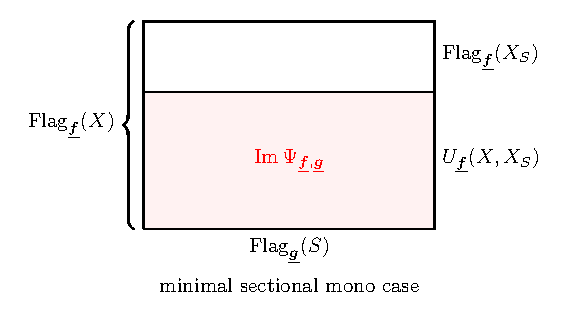
\includegraphics[width=6cm]{figures/space/preferredimage.pdf}
       \end{figure} 
}
%\end{overlayarea}
\end{frame}

\begin{frame}[fragile]{How to find nicer $\eta$?}
\begin{proposition}
For $X \hookrightarrow Y$ minimal sectional mono, the induced SES
\vspace{-3mm}
\[\begin{tikzcd}
\eta: 0 & {X} & {Y} & {S} & 0
\arrow[from=1-1, to=1-2]
\arrow["\iota", from=1-2, to=1-3]
\arrow["\pi", from=1-3, to=1-4]
\arrow[from=1-4, to=1-5]
\end{tikzcd}\]
\\
\vspace{-3mm}
satisfies the condition of Theorem B. Moreover,
\vspace{-3mm}
$$\Img \Psi_{\ftdimvec{f},\ftdimvec{g}} = \begin{cases}
U_{\ftdimvec{f}}(X,X_S), & \ftdimvec{g}_i=\dimv S\\
\;\Flag_{\ftdimvec{f}}(X) \times \Flag_{\ftdimvec{g}}(S),\hspace{15mm}$\,$ & \text{otherwise}
\end{cases}$$

\end{proposition}
\begin{proposition}
In addition, if $X \hookrightarrow Y$ is irreducible mono, then\\[-5mm]
$$X_S=0 \quad \text{ or } \quad X_S \hookrightarrow X \text{ is irreducible mono.}$$
\end{proposition}

\begin{corollary}
For $M \in \ind(Q)$, if exist irreducible mono $X \hookrightarrow M$, then\\[-5mm]
$$\Flag_{d}(M) \text{ has an affine paving.}$$
\end{corollary}
\end{frame}

\begin{frame}[fragile,label=notcurrent]{Process}
\begin{figure}[ht]
    \centering
    \only<1>{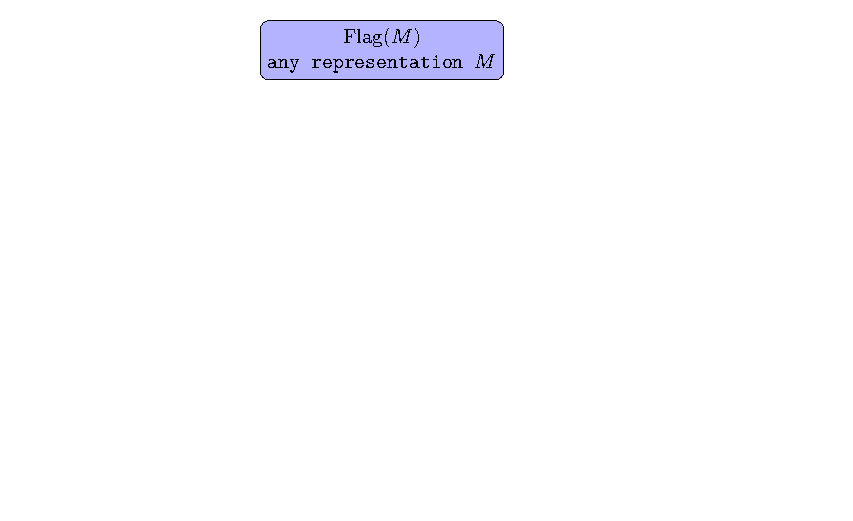
\includegraphics[scale=0.75]{figures/flowchart/flowchart11.pdf}}
    \only<2>{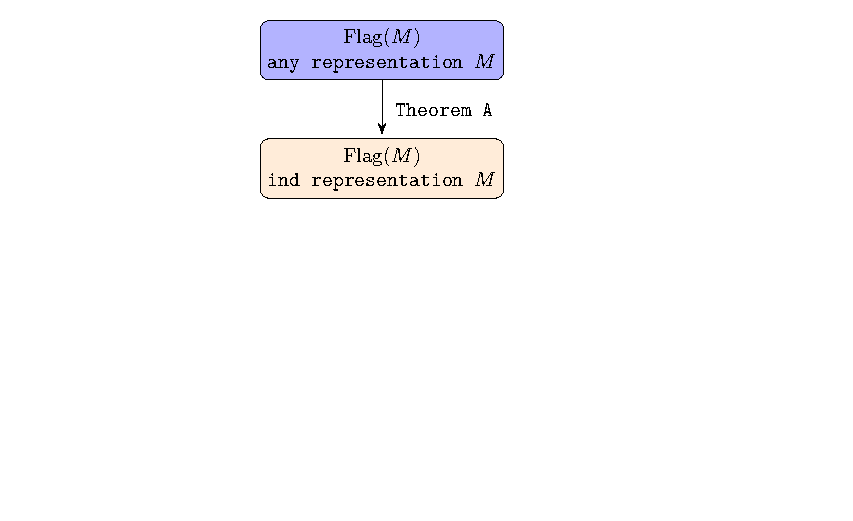
\includegraphics[scale=0.75]{figures/flowchart/flowchart12.pdf}}
    \only<3>{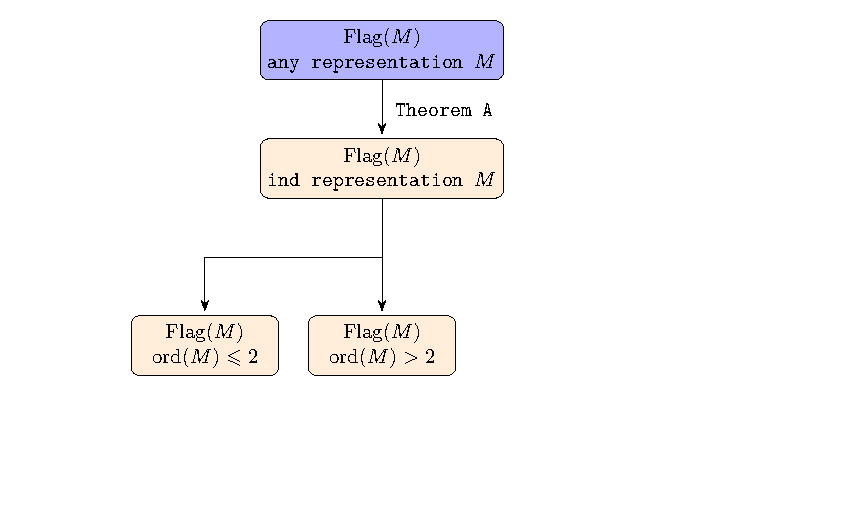
\includegraphics[scale=0.75]{figures/flowchart/flowchart13.pdf}}
    \only<4>{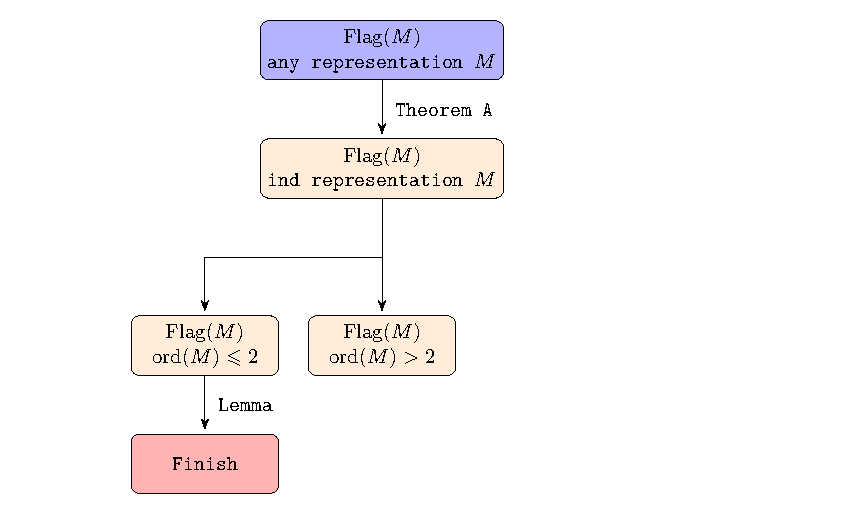
\includegraphics[scale=0.75]{figures/flowchart/flowchart1.pdf}}
    \only<5>{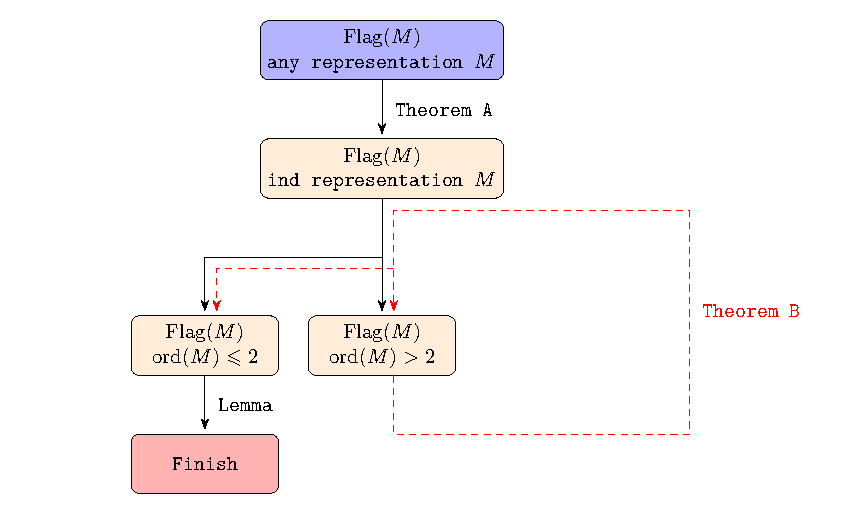
\includegraphics[scale=0.75]{figures/flowchart/flowchart2.pdf}}
    \only<6>{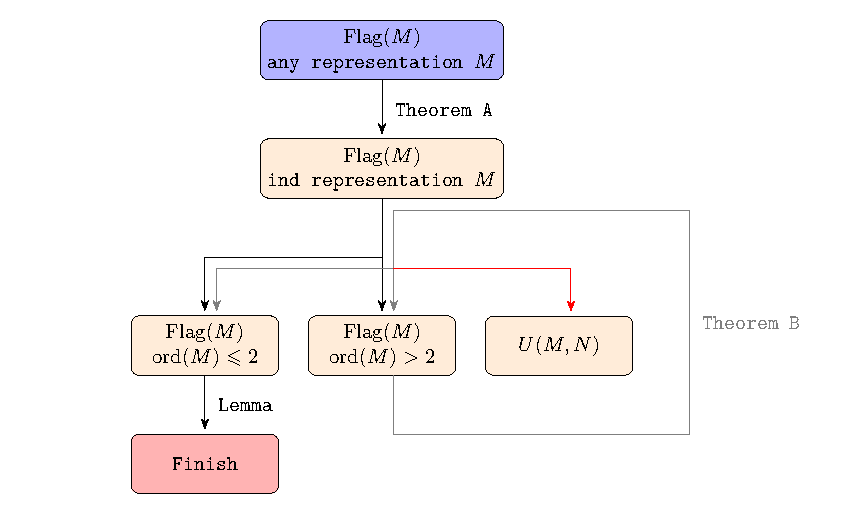
\includegraphics[scale=0.75]{figures/flowchart/flowchart3.pdf}}
    \only<7>{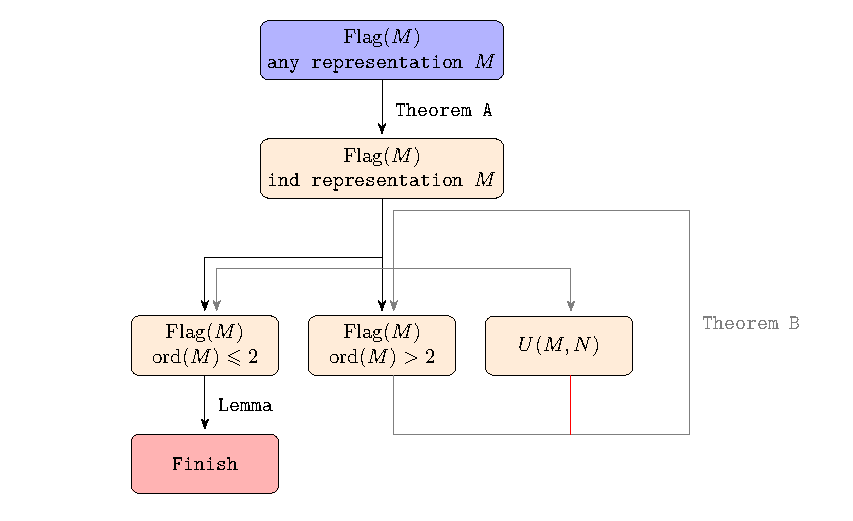
\includegraphics[scale=0.75]{figures/flowchart/flowchart4.pdf}}
%    \caption[The proof of affine paving in Dynkin case]{The process of induction}
%    \vspace{2mm}
    \label{fig:flowchart}
\end{figure}
\end{frame}


\begin{frame}[fragile]{What is remaining?}
\begin{flushleft}

      $E_6$ :\parbox[h][][c]{7cm}{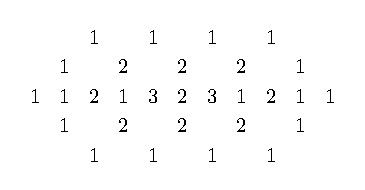
\includegraphics[height=0.28\textheight]{figures/horizontal/h_E6.pdf}}
      \\[-2mm]
      $E_7$ :\parbox[h][][c]{7cm}{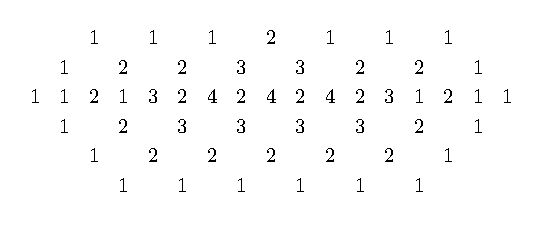
\includegraphics[height=0.32\textheight]{figures/horizontal/h_E7.pdf}}
      \\[-7mm]
      $E_8$ :\parbox[h][][c]{7cm}{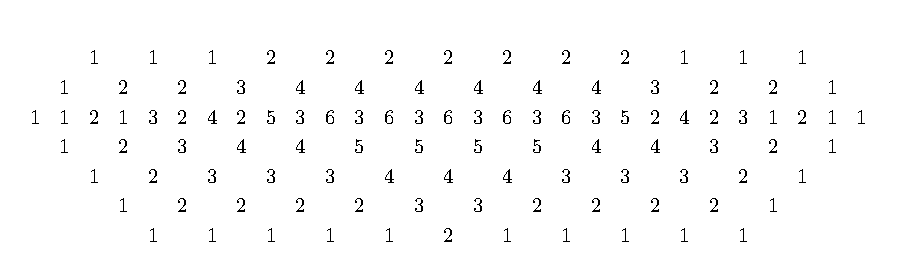
\includegraphics[height=0.37\textheight]{figures/horizontal/h_E8.pdf}}
\end{flushleft}
\end{frame}

\begin{frame}[fragile]{What is remaining?}
\begin{flushleft}

      $E_6$ :\parbox[h][][c]{7cm}{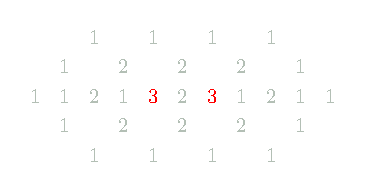
\includegraphics[height=0.28\textheight]{figures/horizontal/h_E6_red.pdf}}
      \\[-2mm]
      $E_7$ :\parbox[h][][c]{7cm}{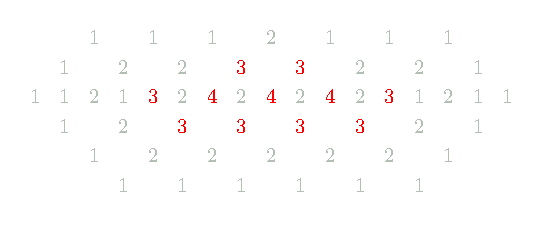
\includegraphics[height=0.32\textheight]{figures/horizontal/h_E7_red.pdf}}
      \\[-7mm]
      $E_8$ :\parbox[h][][c]{7cm}{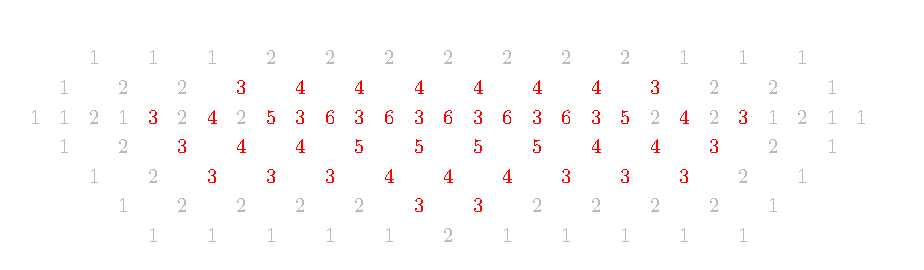
\includegraphics[height=0.37\textheight]{figures/horizontal/h_E8_red.pdf}}
\end{flushleft}
\end{frame}
\begin{frame}[fragile]{What is remaining?}
\begin{flushleft}

      $E_6$ :\parbox[h][][c]{7cm}{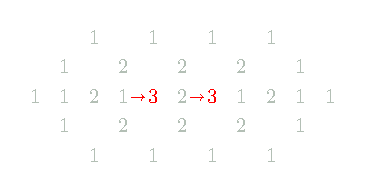
\includegraphics[height=0.28\textheight]{figures/horizontal/h_E6_red_easy.pdf}}
      \\[-2mm]
      $E_7$ :\parbox[h][][c]{7cm}{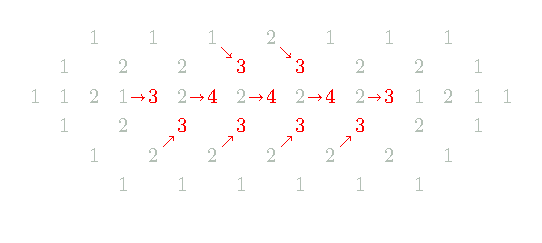
\includegraphics[height=0.32\textheight]{figures/horizontal/h_E7_red_easy.pdf}}
      \\[-7mm]
      $E_8$ :\parbox[h][][c]{7cm}{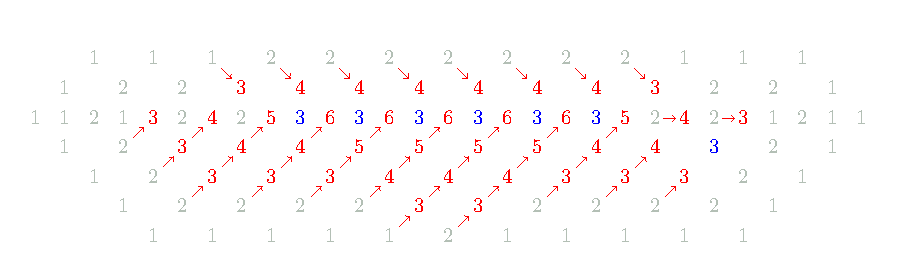
\includegraphics[height=0.37\textheight]{figures/horizontal/h_E8_red_easy.pdf}}
\end{flushleft}
\end{frame}
\end{document}